s%% Description: Local/Global Options of OPC XML-DA
%%
%%


\section {Appendix A - Local/Global OPC Options}
\thispagestyle{plain}

The OPC XML-DA specification defines various options, which can be
global and/or local and are associated with one or more OPC operations.
A detailed description of these options can be found in \cite{OPCXMLDA}.
However, the specification is somehow complicated and some of these
options can not be easily found. Moreover these options will be 
represented by specific Python data types.

In order to ease the client/server development with PyOPC, table
\ref{operations1} and \ref{operations2} outline what options are
used by which functions. The letters ``G'' and ``L'' indicate if the
option is global or local for an OPC operation.

\begin{table}[!ht]
\htmlborder{1}
\centering
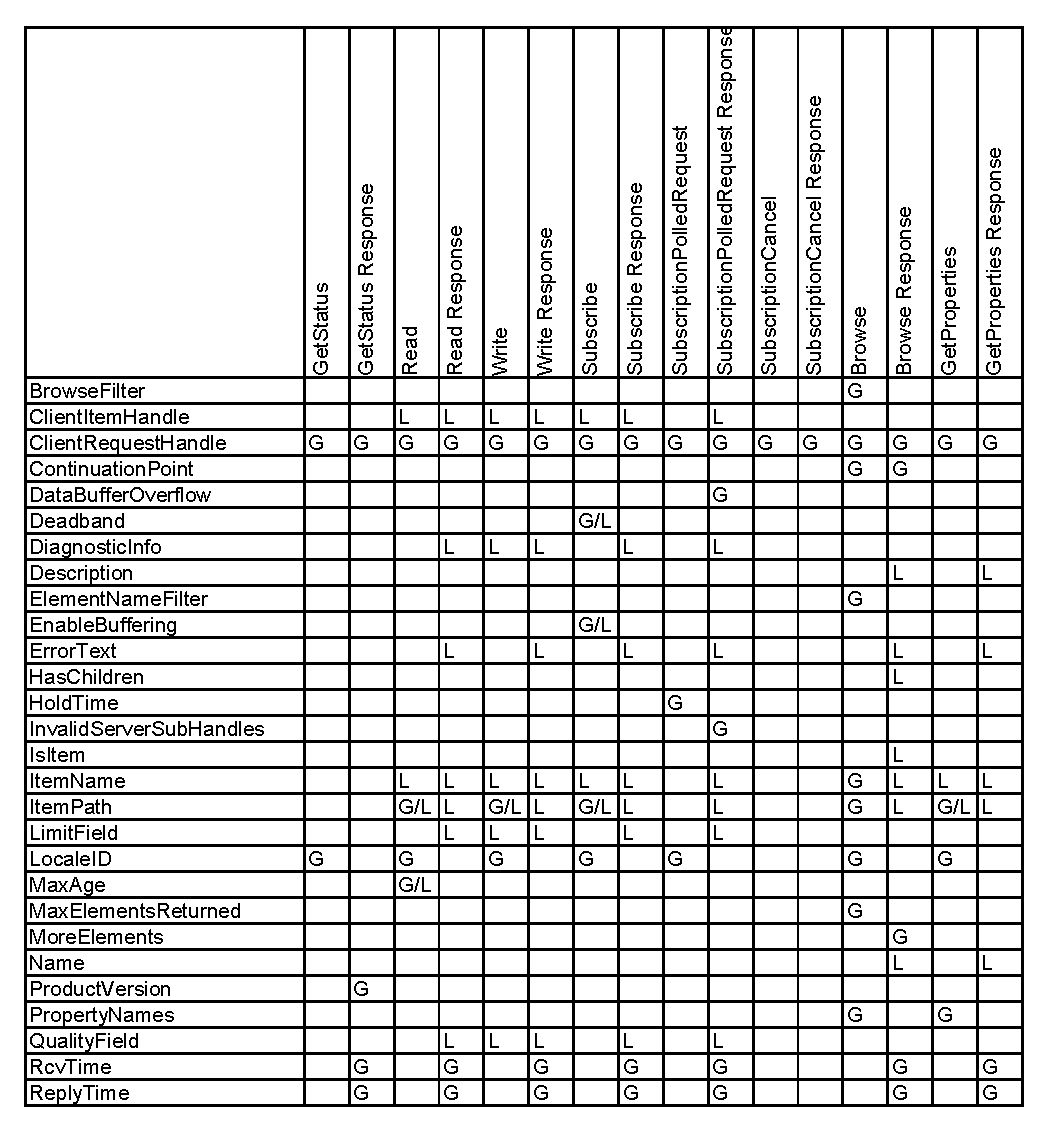
\includegraphics[scale=0.9]{graphics/operations1.eps}
\caption{OPC Options and Operations}
\label {operations1} 
\end{table}

\begin{table}[!ht]
\htmlborder{1}
\centering
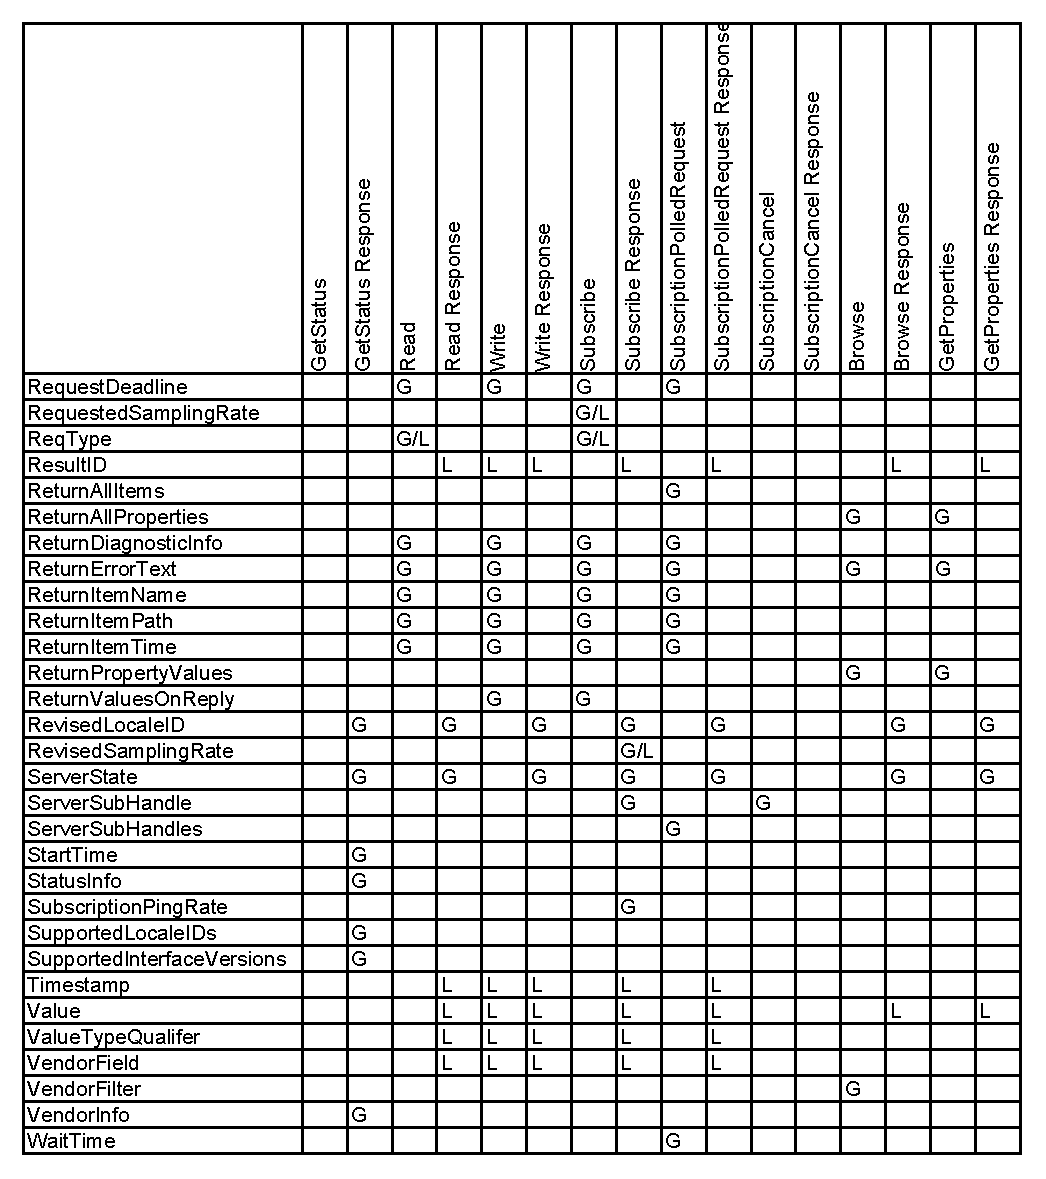
\includegraphics[scale=0.9]{graphics/operations2.eps}
\caption{OPC Options and Operations}
\label {operations2} 
\end{table}

Moreover an alphabetical reference of all available OPC options is
given in this appendix, which outlines the functionality of an OPC
option and moreover denotes, by which Python data type it is
represented in the PyOPC framework.


\begin{description}

\item[BrowseFilter] ({\sl string}) Limits the returned elements during
a browse operation. Allowed values are {\sl all, branch, item}.
\item[ClientItemHandle] ({\sl string}): An identifier of the item in a
request message. The ClientItemHandle is returned along with the
requested item.
\item[ClientRequestHandle] ({\sl string}): An identifier of the client
request.
\item[ContinuationPoint] ({\sl string}): A browse option for specifying
secondary browse requests.
\item[DataBufferOverflow] ({\sl bool}): Indicates if some item changes
were lost during subsequent subscription polls
\item[Deadband] ({\sl float}): The percentage of an item value change
which has to be exceeded so that the item ``has changed'', meaning
that the item will be sent during the next subscription poll.
\item[DiagnosticInfo] ({\sl string}): Additional server specific
information in case of an error.
\item[Description] ({\sl string}): A verbose description of an item
property
\item[ElementNameFilter] ({\sl string}): Limits the returned elements
during a browse operation
\item[EnableBuffering] ({\sl bool}): Denotes if changed values should
be buffered in case of a subscription
\item[ErrorText] ({\sl string}): Verbose error description in case of
an item error
\item[HasChildren] ({\sl bool}): Indicates if a browse element has
child elements
\item[HoldTime] ({\sl datetime}): Time to wait until the subscription poll
response is sent
\item[InvalidServerSubHandles] ({\sl list of strings}): A list of invalid
ServerSubHandles
\item[IsItem] ({\sl bool}): Indicates if a browse element is an item
\item[ItemName] ({\sl string}): The ItemName is part of the namespace
of an OPC item. Together with the ItemPath, it forms a unique
identification of an item.
\item[ItemPath] ({\sl string}): The ItemPath is part of the namespace
of an OPC item. Together with the ItemName, it forms a unique
identification of an item.
\item[LimitField] ({\sl string}): Transports the limit status of an
OPC item and may be one of the following string: {\sl none, low,
high, constant}.
\item[LocaleID] ({\sl string}): Requested locale for the return message.
\item[MaxAge] ({\sl long}): Denotes how old the item value may be in
milliseconds. MaxAge can be utilized for item caching in the server.

% A newpage is inserted as otherwise the inserted table leads to the 
% placement of the word ``request'' on the next page, which looks weird.
\newpage

\item[MaxElementsReturned] ({\sl long}): Maximum amount of returned
elements during a browse request.
\item[MoreElements] ({\sl bool}): Indicates that there are more
elements than the returned ones in a browse response message
\item[Name] ({\sl string/QName}): This option is used as an identifier
for a browse element (string type) or a property (QName type).
\item[ProductVersion] ({\sl string}): A version string of the OPC server
\item[PropertyNames] ({\sl list of QNames}): A list of item properties
that should be returned.
\item[QualityField] ({\sl string}): The quality of an OPC item value.
\cite{OPCXMLDA} specifies a predefined list of allowed qualities, such
as ``good'', ``uncertain'' or ``bad''.
\item[RcvTime] ({\sl datetime}): The time the server received the request.
\item[ReplyTime] ({\sl datetime}): The time the server returned the response.
\item[RequestDeadline] ({\sl datetime}): The time until the server
response has to be issued.
\item[RequestedSamplingRate] ({\sl long}): The time in milliseconds in
which the server checks for value changes in case of a subscription.
\item[ReqType] ({\sl QName}): With this options, the client may
specify the data type of an OPC item value. The available data types
are listed in \cite{OPCXMLDA}.
\item[ResultID] ({\sl QName}): In case of an item error, this option
specifies the error type.
\item[ReturnAllItems] ({\sl bool}): Indicates if the server should
return only the changed or all OPC items during a subscription poll
\item[ReturnAllProperties] ({\sl bool}): Indicates if all item
properties should be returned
\item[ReturnDiagnosticInfo] ({\sl bool}): Return additional server
specific information in case of an error
\item[ReturnErrorText] ({\sl bool}): If True, the OPC server returns a
verbose error description in case of an item error.
\item[ReturnItemName] ({\sl bool}): Indicates whether the ItemName
is returned by the server
\item[ReturnItemPath] ({\sl bool}): Indicates whether the ItemPath is
returned by the server
\item[ReturnItemTime] ({\sl bool}): Indicates whether the Timestamp of an
OPC item is returned by the server
\item[ReturnPropertyValues] ({\sl bool}): Indicates whether all item
property values should be included in a response message
\item[ReturnValuesOnReply] ({\sl bool}): Specifies if the item values
should be included in the response message
\item[RevisedLocaleID] ({\sl string}): In case the requested locale is not
implemented by the server, it is revised. The revised locale is sent back
to the client by the RevisedLocaleID option.
\item[RevisedSamplingRate] ({\sl long}): If the OPC server does not
the requested subscription sampling rate, it returns a revised rate in
this option.
\item[ServerState] ({\sl string}): The current status of the OPC
server, the values may be one of the following: {\sl running, failed,
noConfig, suspended, test, commFault}
\item[ServerSubHandle] ({\sl string}): An identifier of an OPC
subscription
\item[ServerSubHandles] ({\sl list of strings}): A list of
ServerSubHandles.
\item[StartTime] ({\sl datetime}): The time the OPC server was started
\item[StatusInfo] ({\sl string}): Provides additional server information.
\item[SubscriptionPingRate] ({\sl long}): Maximum time in milliseconds
between SubscriptionPolledRequest operations. If the ping rate is
exceeded, the subscription will be canceled.
\item[SupportedLocaleIDs] ({\sl string}): String that contains all
supported locales by the server
\item[SupportedInterfaceVersions] ({\sl string}): Supported versions
of the OPC XML-DA standard, currently only ``XML\_DA\_Version\_1\_0'' is
allowed
\item[Timestamp] ({\sl datetime}): The time when the OPC item value
was sampled
\item[Value] ({\sl anyType}): The value of an OPC item or OPC
property
\item[ValueTypeQualifier] ({\sl QName}): In case the value is
date/time based, it will identifiy the exact XML-Schema data type.
\item[VendorField] ({\sl long}): A numeric value that matches the OPC
Vendor Bit Field
\item[VendorFilter] ({\sl string}): Limits the returned elements
during a browse operation
\item[VendorInfo] ({\sl string}): Vendor specific server information
\item[WaitTime] ({\sl long}): Time in milliseconds which the server
should wait during a pending subscription poll for item value changes
\end{description}

